\documentclass{standalone}
\usepackage{tikz}

\begin{document}

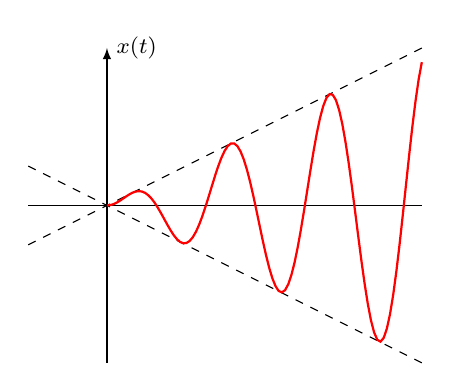
\begin{tikzpicture}[>=latex]
	\draw (-1,0) -- (4,0);
	\draw [->] (0,-2) -- (0,2) node [right] {\footnotesize \(x(t)\)};
	\draw [dashed, domain=-1:4] plot(\x , {0.5*\x});
	\draw [dashed, domain=-1:4] plot(\x , {-0.5*\x});
	\draw [thick , red , domain=0:4, samples = 100] plot(\x , {0.5*sin(5*\x r) *\x});
\end{tikzpicture}

\end{document}
